\documentclass[sigconf,review,anonymous,nonacm]{acmart}

\settopmatter{printacmref=false,printfolios=true,printccs=false}
\renewcommand\footnotetextcopyrightpermission[1]{}
\pagestyle{plain}

\usepackage{booktabs}
\usepackage{tabularx}
\usepackage{multirow}
\usepackage{makecell}
\usepackage{amsmath}
\usepackage{enumitem}
\usepackage{graphicx}
\usepackage{array}
\usepackage{xspace}

\graphicspath{{./}}

\newcommand{\skillability}{\textit{skillability}\xspace}
\newcommand{\sscore}{\textit{SS}\xspace}

\title{From Software Repositories to Agent Skills: An Exploratory Empirical Study of Skillability in Open-Source Ecosystems}

\author{Anonymous Authors}
\affiliation{
  \institution{Anonymous Institution(s)}
  \country{}
}

% \acmConference[ICSE '26]{International Conference on Software Engineering}{2026}{}
% \acmBooktitle{Proceedings of the International Conference on Software Engineering (ICSE '26)}
\acmYear{2026}
\acmDOI{}
\acmISBN{}

\begin{document}

\begin{abstract}
AI agent ecosystems increasingly rely on reusable ``skills,'' but deciding which open-source software projects are worth converting into skills remains largely ad hoc. We present an exploratory empirical study of 29,896 artifacts: 2,200 skills from the Clawhub marketplace and 27,696 GitHub repositories sampled from a larger filtered corpus. We operationalize \skillability as a six-dimensional construct spanning task clarity, interface clarity, composability, automation value, deployment friction, and operational risk, and annotate artifacts with an LLM-based pipeline over metadata and README excerpts, validated on a 200-item human-coded subsample (87\% agreement within $\pm$0.5 points).

The results reveal a large and structured conversion frontier. Marketplace skills score substantially higher than sampled GitHub repositories (3.75 vs.\ 2.88; $\Delta=0.87$, Welch's $t$-test $p<0.001$, Cohen's $d=0.74$), and 35.8\% of all analyzed artifacts satisfy our high-\skillability threshold. High-\skillability candidates concentrate in Data Retrieval \& Search, Multimedia Content, and System Infrastructure, while raw \skillability is effectively independent of repository popularity (Spearman $r_s=0.003$). Using \skillability together with lightweight repository-quality signals, we identify 9,033 GitHub repositories as promising skill-conversion candidates.

We position the paper as a scalable empirical foundation for repository-to-skill pipelines rather than as a finalized measurement paper. The contribution is a reusable rubric, a large-scale characterization of agent-facing software, and concrete evidence that open-source ecosystems contain enough high-potential repositories to make systematic and potentially batch-oriented skillification a realistic next step. The project website link is https://red0orange.github.io/repo2skill.
\end{abstract}

\keywords{AI agents, software reuse, repository mining, skill marketplaces, empirical software engineering}

\maketitle

\section{Introduction}

Large language model based agents are changing how software is consumed. Instead of calling libraries directly or integrating APIs manually, agents increasingly rely on higher-level tools and ``skills'' that expose useful capabilities through descriptions, schemas, and invocation interfaces [1,2]. This shift creates a new software engineering problem: some software projects are much easier than others to expose as agent-usable skills, but we still lack systematic ways to identify them at scale.

Today, skill creation is mostly opportunistic. Developers manually browse open-source repositories, select projects that appear useful for agents, wrap them with platform-specific interfaces, and publish them to marketplaces such as Clawhub or MCP-based registries [34,35]. That workflow does not scale well. GitHub hosts an enormous supply of potentially reusable software [3], but only a small fraction has been adapted for agent use. For marketplace operators, this means missing high-value capabilities. For software developers, it means little guidance on what design choices make a project more agent-friendly.

This paper studies that gap through the lens of \skillability: the extent to which a software project appears suitable for transformation into an agent-facing skill. We intentionally frame \skillability as an exploratory construct rather than a finalized quality metric. Our goal is not to present a finished measurement instrument, but to provide a structured and scalable basis for the next stage of work: discovering, prioritizing, and eventually industrializing the conversion of open-source repositories into agent-usable skills.

The distinction matters. A repository can be high quality, influential, and technically sophisticated while still being a poor candidate for packaging as a standalone skill. The Linux kernel is indispensable software, but its broad scope, operational risk, and deep environment coupling make it difficult to expose as a focused agent skill. By contrast, tools such as \texttt{jq} or \texttt{fzf} have narrow purposes, clear interfaces, and immediate automation value. Traditional indicators such as stars or community size do not capture this difference well.

From a software engineering perspective, the problem sits at the intersection of software reuse, API usability, repository mining, and emerging agent ecosystems [4,5,13,27]. Prior work has studied reusable components, software ecosystems, and tool use in LLM agents, but there is still little empirical evidence on what kinds of open-source software are most amenable to agent-facing reuse. That is the gap we address.

We make four contributions:
\begin{enumerate}[leftmargin=*,itemsep=2pt]
    \item We operationalize an exploratory six-dimensional \skillability construct that captures task clarity, interface clarity, composability, automation value, deployment friction, and operational risk.
    \item We build and analyze a 29,896-artifact dataset spanning both an agent skill marketplace and sampled GitHub repositories, using LLM-assisted annotation with human spot validation.
    \item We report ecosystem-scale findings on how \skillability is distributed across repositories, domains, languages, and granularities, showing that promising candidates are concentrated rather than rare.
    \item We derive a practical opportunity-ranking heuristic and identify concrete high-potential repository candidates for skill transformation, establishing an actionable starting point for large-scale or semi-automated repository-to-skill conversion pipelines.
\end{enumerate}

\section{Background and Related Work}

\subsection{Software Reuse and Componentization}

Software reuse has been a core concern of software engineering since McIlroy's call for mass-produced software components [4]. Component-based development and related paradigms emphasize encapsulation, interface contracts, and composability [5,6,7]. Empirical work on reuse has repeatedly highlighted clear specifications, stable interfaces, modularity, and low coupling as enabling factors [8,9,10]. Our study builds on that tradition, but shifts the consumer from a human developer to an autonomous or semi-autonomous agent.

This shift changes the operational requirements of reuse. An agent-facing component must not only be functionally reusable; it must also be easy for a model to discover, understand from textual and structured descriptions, and invoke safely. These are not identical to classical reuse concerns, even though they overlap.

\subsection{Software Ecosystems and Repository Mining}

Software ecosystem research studies collections of interdependent projects, developers, and users that evolve in a shared environment [13,14]. Repository mining has provided methods for characterizing large corpora, measuring project health, and identifying suitable samples for empirical studies [15,16,17,18,19]. Our work adopts that empirical mindset, but focuses on a new selection problem: which repositories appear especially promising for downstream reuse in agent ecosystems.

This problem is close to, but distinct from, repository popularity prediction or quality assessment. Popular repositories may be broad platforms, frameworks, or applications whose value does not translate into skill packaging. Conversely, small but focused tools may be highly promising. The study therefore complements prior mining work by introducing a different target construct.

\subsection{API Usability, Tool Use, and Agent Interfaces}

API usability research shows that interface design strongly affects learnability, adoption, and developer productivity [22,23,24,25,26]. Many of the same principles matter for agent consumption: explicit parameters, predictable behavior, and good documentation reduce ambiguity during tool selection and invocation. Recent work on LLM tool use, including Toolformer, ReAct, Gorilla, and related systems, has focused primarily on the agent side of the problem [27,28,29,33]. Our study complements that literature by looking at the software side: what properties of a software artifact make it easier to expose as a tool in the first place.

\subsection{Skill Marketplaces and Emerging Agent Ecosystems}

Skill marketplaces such as Clawhub and standards such as the Model Context Protocol represent early infrastructure for distributing agent-usable capabilities [34,35]. These ecosystems face curation, recommendation, and duplication problems that resemble app stores and package registries, but with an important difference: the primary consumer may be an automated agent rather than a human user [36,37,38]. This raises new questions about discoverability and interface semantics that conventional marketplace quality signals may not capture.

\subsection{Measurement and LLM-Based Annotation}

Software measurement research emphasizes construct validity, reliability, and the need to avoid overclaiming beyond what an instrument can support [41,42]. These concerns are especially important here because \skillability is not yet a mature construct. At the same time, large-scale annotation of tens of thousands of repositories is impractical without automation. Recent work suggests that LLMs can support annotation and evaluation workflows efficiently, though concerns remain about bias, consistency, and validity [43,44,45]. Our study adopts LLM-assisted coding for scale, but treats the results as exploratory evidence and explicitly discusses the threats this introduces.

\subsection{Gap and Positioning}

Taken together, prior work gives us strong foundations for studying software reuse, interfaces, and ecosystems, but leaves three gaps. First, the literature does not yet provide an agent-centric characterization of reusable software components. Second, empirical evidence on skill marketplaces remains limited. Third, current skill discovery practices are still ad hoc. We position this paper as an exploratory empirical study that addresses those gaps by operationalizing a preliminary construct and using it to characterize a large cross-ecosystem corpus.

\section{Study Design}

\subsection{Research Questions}

We study four research questions:
\begin{description}[leftmargin=0.5cm,style=nextline]
    \item[RQ1.] How can software be characterized for agent-facing reuse?
    \item[RQ2.] How do marketplace skills differ from sampled GitHub repositories?
    \item[RQ3.] Where are high-\skillability projects concentrated?
    \item[RQ4.] Which repositories appear most promising for skill transformation?
\end{description}

\subsection{Skillability Construct}

We define \skillability using six dimensions scored on a 1--5 scale: Task Clarity (TC), Interface Clarity (IC), Composability (C), Automation Value (AV), Deployment Friction (DF), and Operational Risk (OR). For DF and OR, higher raw scores mean worse conditions, so we reverse-code them before aggregation:

\begin{equation}
\begin{aligned}
\mathrm{DF}' &= 6 - \mathrm{DF}\\
\mathrm{OR}' &= 6 - \mathrm{OR}\\
\sscore &= 0.25\mathrm{TC} + 0.20\mathrm{IC} + 0.20\mathrm{C} + 0.25\mathrm{AV} + 0.05\mathrm{DF}' + 0.05\mathrm{OR}'
\end{aligned}
\end{equation}

This keeps the overall score in the range $[1,5]$ because the weights sum to 1.0 and all aggregated dimensions are oriented in the same direction. We use \(\sscore \ge 4.0\) as a practical high-\skillability threshold. We treat that threshold as an analysis cutoff rather than a validated boundary.

\subsection{Capability Taxonomy}

To support domain-level analysis, we classify each project into one of ten primary capability categories plus an ``Other'' bucket:
\begin{enumerate}[leftmargin=*,itemsep=1pt]
    \item Code \& DevOps
    \item Data Retrieval \& Search
    \item Document Processing
    \item Web Automation
    \item Communication \& Collaboration
    \item Knowledge \& Workflow
    \item Business \& Productivity
    \item Multimedia Content
    \item System Infrastructure
    \item External Service Connectors
\end{enumerate}

We also record artifact granularity (primitive tool, service wrapper, workflow skill, platform adapter) and execution mode (local deterministic, remote API mediated, browser mediated, human in the loop, hybrid).

\subsection{Dataset Construction}

We combined two data sources. For Clawhub, we collected metadata and skill specifications for 22,413 skills as of March 2026 and drew a 2,200-item stratified sample. For GitHub, we collected 347,860 repositories and filtered them to repositories with at least 10 stars, activity within the previous two years, a README file, and non-archived status. We then drew a 27,700-item stratified sample and retained 27,696 valid annotations after response filtering.

The study therefore analyzes 29,896 artifacts in total. Our scope is intentionally narrower than ``all software projects'': the sampling frame emphasizes active, documented, community-visible artifacts. This is appropriate for identifying realistic conversion candidates, but it limits generalizability.

\begin{table}[t]
\caption{Dataset overview}
\label{tab:dataset}
\centering
\begin{tabular}{lrrr}
\toprule
Metric & Clawhub & GitHub & Total \\
\midrule
Projects & 2,200 & 27,696 & 29,896 \\
Mean stars & 847 & 1,843 & 1,770 \\
Median stars & 156 & 127 & 129 \\
Languages & 42 & 87 & 89 \\
Capability categories & 10 + Other & 10 + Other & 10 + Other \\
\bottomrule
\end{tabular}
\end{table}

\subsection{LLM-Assisted Annotation and Validation}

We used Alibaba Qwen-Plus (\texttt{qwen-plus-2024-11}) to score each artifact and assign taxonomy labels. Each prompt included repository metadata, a README excerpt capped at 3,000 characters, a detailed scoring rubric, and a constrained JSON schema. We used temperature 0.1, schema validation, and retry logic for malformed outputs. The pipeline produced valid outputs for 29,896 of 29,900 sampled artifacts (99.99\%).

We conducted a spot-validation study on 200 randomly sampled artifacts (100 Clawhub, 100 GitHub). Two human annotators independently applied the same rubric and compared their judgments with the model outputs. The LLM agreed with the human reference within $\pm$0.5 points in 87\% of cases overall. Per-dimension agreement ranged from 84\% (Composability) to 91\% (Automation Value). This validation is useful but limited: it is not a full reliability study, and it does not establish convergent or predictive validity in the measurement-theory sense.

\subsection{Analysis Procedures}

We use four analysis procedures aligned with the research questions:
\begin{enumerate}[leftmargin=*,itemsep=2pt]
    \item Descriptive characterization of distributions, means, and high-\skillability rates.
    \item Cross-group comparison using Welch's $t$-test, confidence intervals, and Cohen's $d$.
    \item Association analysis using Spearman correlation for star-related analyses.
    \item Opportunity ranking for GitHub repositories using
\end{enumerate}

\begin{equation}
\mathrm{OpportunityScore} = 0.6 \times \mathrm{normalize}(\sscore) + 0.4 \times \mathrm{RepoQuality}
\end{equation}

\noindent where \(\mathrm{RepoQuality}\) combines log-scaled stars, recency, README length, and license presence. We use this score as a practical prioritization device for downstream conversion workflows rather than as a standalone scientific claim about repository value.

\section{Results}

\subsection{RQ1: Characterizing Skillability}

Across all 29,896 artifacts, the mean \skillability score is 2.95 (SD = 1.18). A total of 10,698 artifacts (35.8\%) satisfy \(\sscore \ge 4.0\).

\begin{figure}[t]
    \centering
    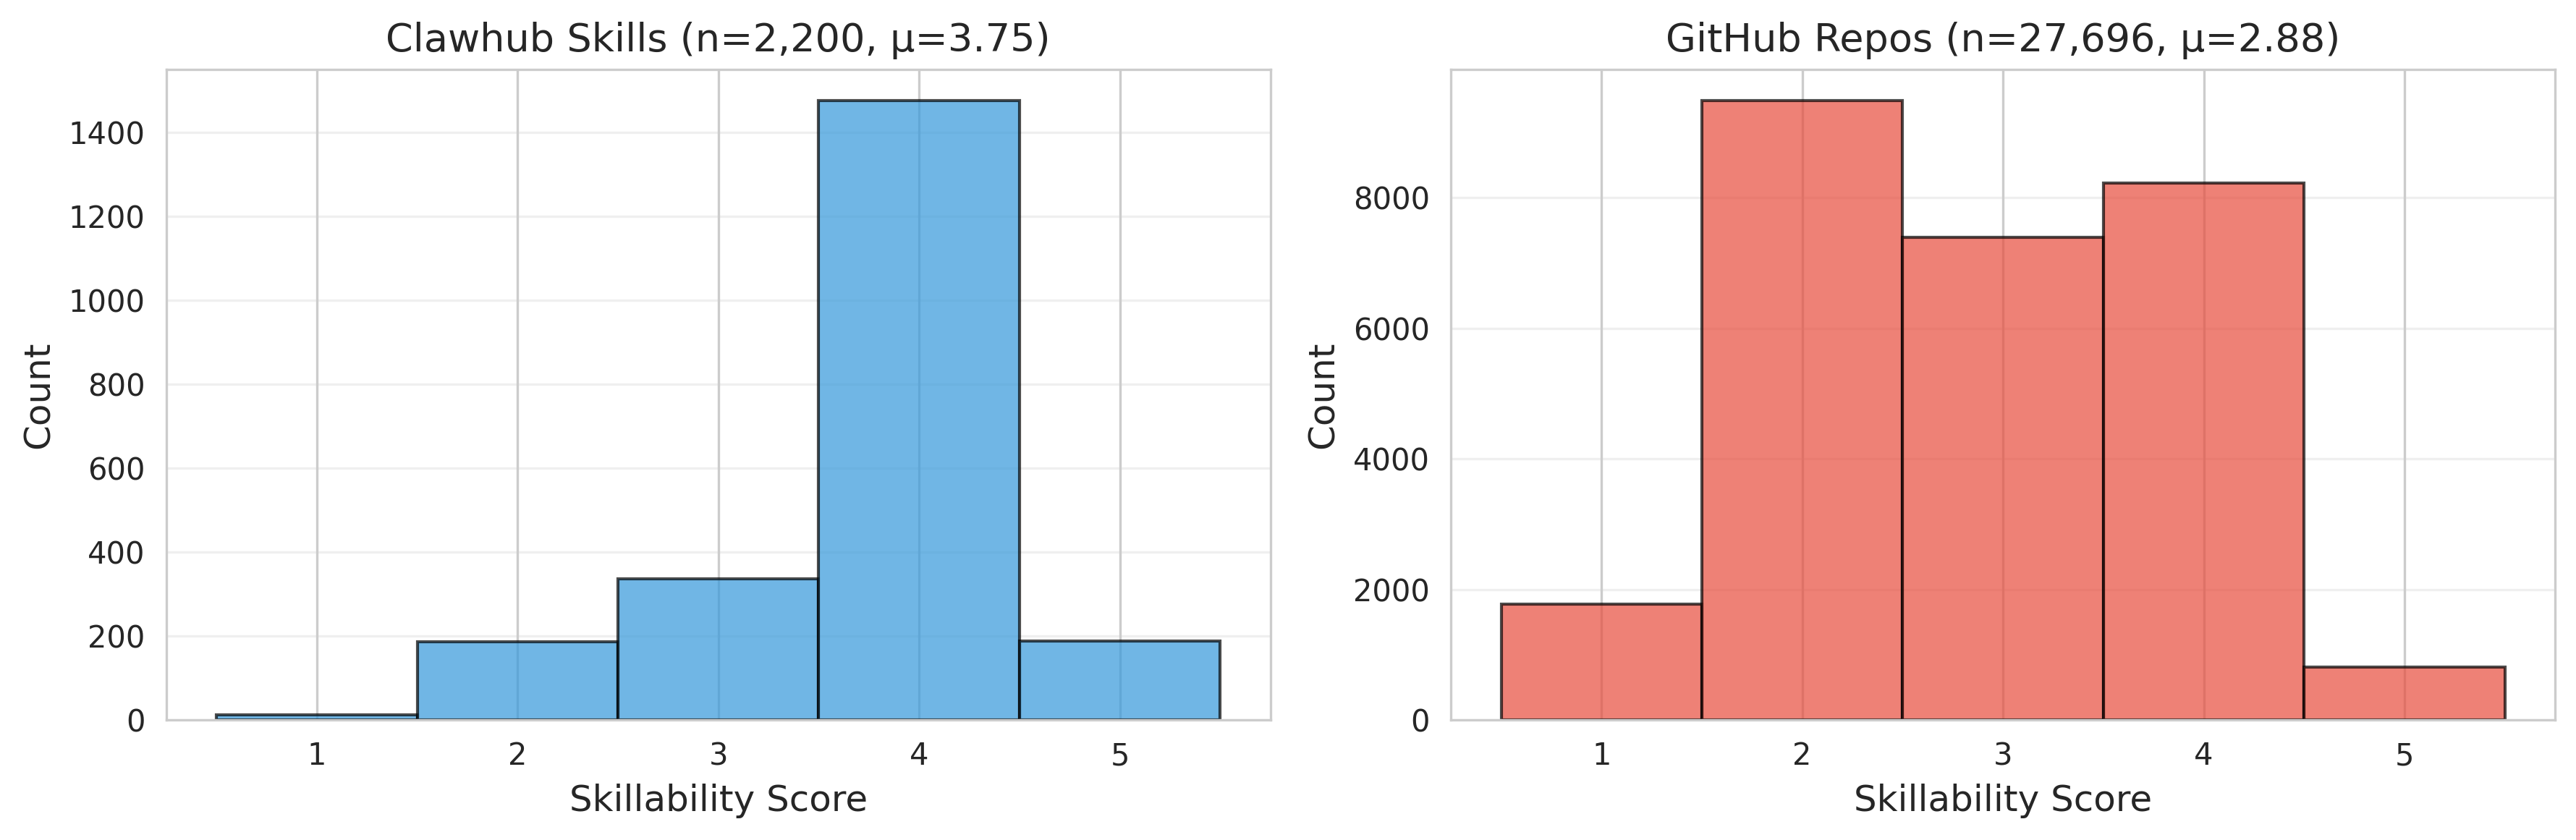
\includegraphics[width=\linewidth]{fig1_skillability_distribution.png}
    \caption{Skillability-score distributions for Clawhub skills and sampled GitHub repositories.}
    \Description{Distribution plot comparing Clawhub and GitHub skillability scores.}
    \label{fig:distribution}
\end{figure}

Figure~\ref{fig:distribution} shows the overall score distributions for Clawhub and GitHub. The Clawhub distribution is concentrated in the upper-middle range, whereas GitHub repositories span the full scale more broadly.

\begin{table*}[t]
\caption{Dimension-level statistics}
\label{tab:dimensions}
\centering
\begin{tabular}{lrrrrrr}
\toprule
Dimension & Mean & SD & Clawhub mean & GitHub mean & $\Delta$ (Clawhub $-$ GitHub) & Cohen's $d$ \\
\midrule
Task Clarity & 4.07 & 0.95 & 4.49 & 4.03 & +0.46 & 0.49 \\
Interface Clarity & 3.67 & 0.93 & 3.84 & 3.66 & +0.18 & 0.19 \\
Composability & 2.81 & 0.94 & 3.42 & 2.76 & +0.66 & 0.70 \\
Automation Value & 3.43 & 1.09 & 4.40 & 3.36 & +1.04 & 0.95 \\
Deployment Friction & 3.21 & 0.84 & 2.98 & 3.23 & -0.25 & -0.30 \\
Operational Risk & 2.71 & 1.08 & 2.90 & 2.69 & +0.21 & 0.19 \\
\bottomrule
\end{tabular}
\end{table*}

Table~\ref{tab:dimensions} reports the per-dimension statistics. For the negatively oriented raw dimensions (Deployment Friction and Operational Risk), lower values are better. Three descriptive patterns stand out. First, Task Clarity is high across the corpus, suggesting that many repositories communicate a focused purpose even when they are not ideal skill candidates. Second, Automation Value shows the largest marketplace-repository gap, which fits the intuition that packaged skills are often created for repetitive high-value tasks. Third, Composability also differentiates the two groups strongly, consistent with marketplace artifacts being intentionally wrapped for integration.

\begin{figure}[t]
    \centering
    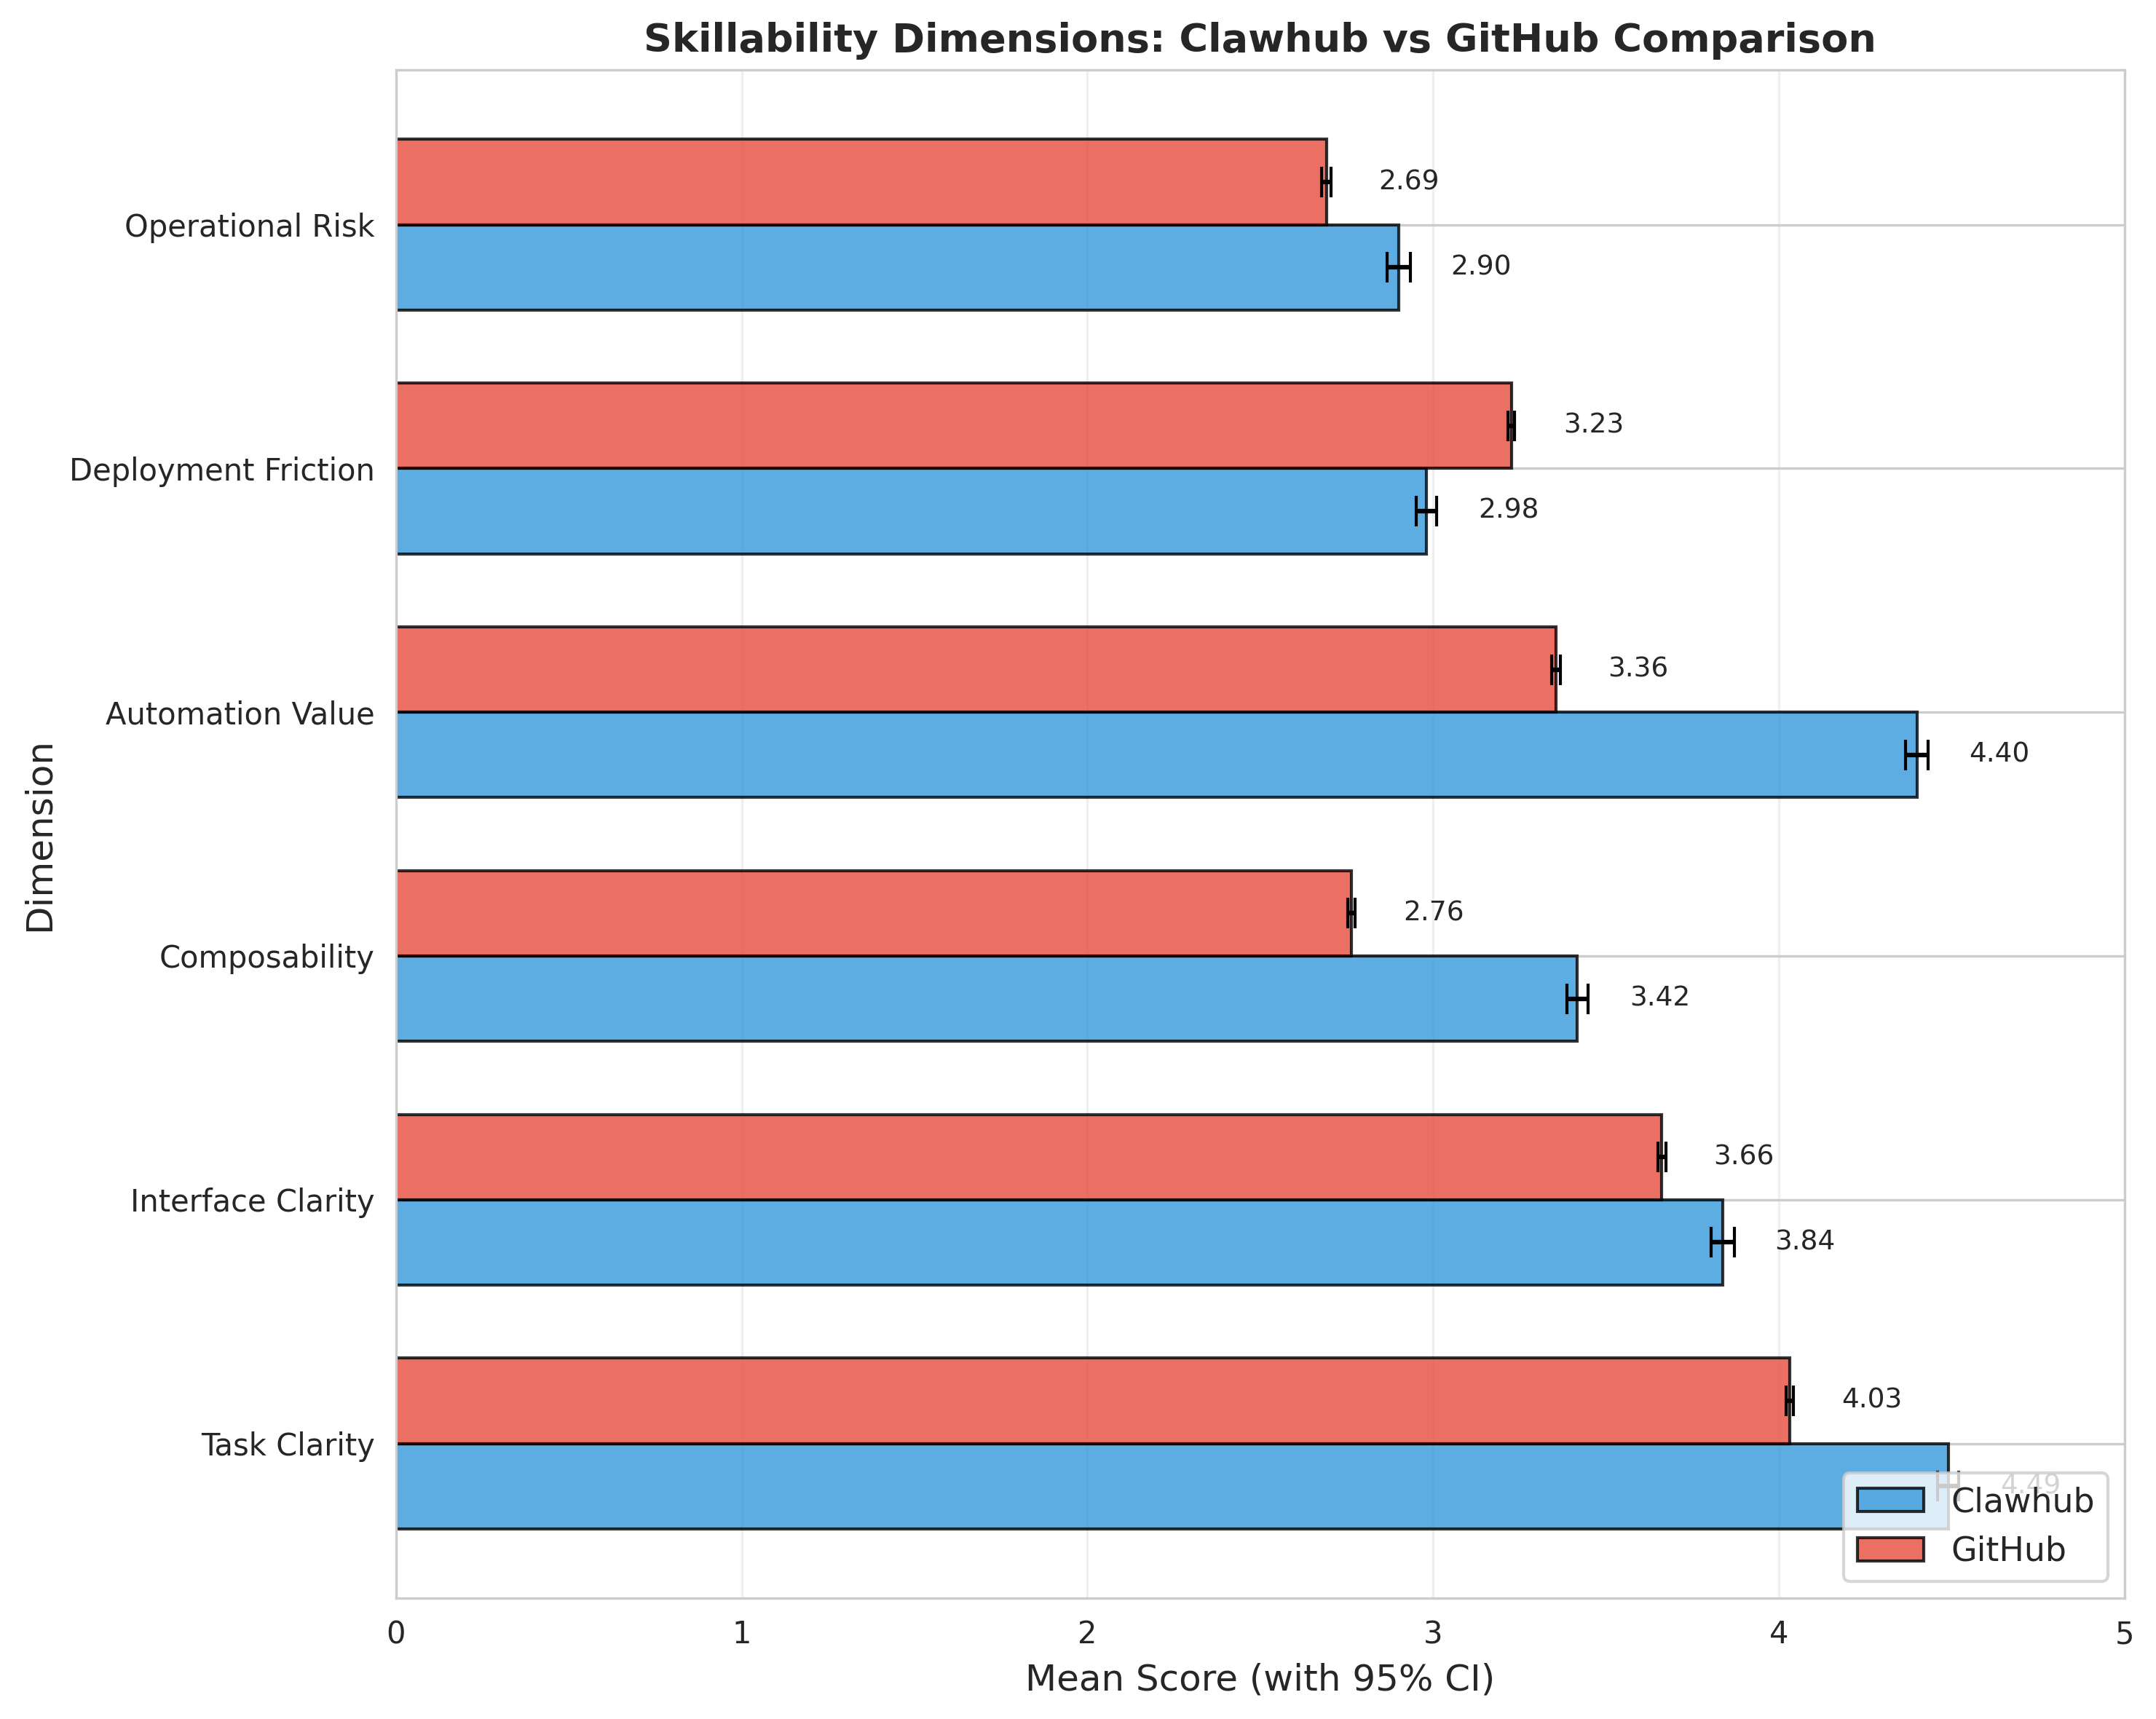
\includegraphics[width=\linewidth]{fig_new1_dimension_comparison_ci.png}
    \caption{Mean scores for the six skillability dimensions in Clawhub and GitHub, with 95\% confidence intervals.}
    \Description{Point-range plot comparing six skillability dimensions between Clawhub and GitHub.}
    \label{fig:dimensions}
\end{figure}

Figure~\ref{fig:dimensions} presents the same comparison with confidence intervals. We also computed descriptive correlations between each raw dimension and the composite score: Automation Value (0.850), Task Clarity (0.805), Composability (0.767), Interface Clarity (0.686), Deployment Friction (-0.080), and Operational Risk (-0.099). These numbers are best read as a sanity check on the weighting scheme, not as independent empirical findings.

\subsection{RQ2: Marketplace Skills vs.\ GitHub Repositories}

Clawhub skills have a mean \skillability of 3.75 (SD = 0.82), whereas sampled GitHub repositories average 2.88 (SD = 1.21). The mean difference is 0.87 with 95\% CI [0.81, 0.93]; Welch's $t$-test yields $p<0.001$, and the effect size is Cohen's $d=0.74$. Bootstrap confidence intervals closely match the parametric interval.

The high-\skillability rate also differs markedly: 75.7\% of Clawhub skills and 32.6\% of GitHub repositories score at least 4.0. This difference is substantial, but it is not clean evidence that marketplace artifacts are inherently ``better software.'' The comparison is confounded by documentation quality, marketplace selection, and artifact scope. We therefore interpret RQ2 as a descriptive ecosystem contrast rather than a causal comparison.

\subsection{RQ3: Where High-Skillability Projects Concentrate}

We next examine where promising projects cluster in the GitHub sample. Table~\ref{tab:categories} shows the distribution by capability category. Data Retrieval \& Search, Multimedia Content, and System Infrastructure exhibit the highest mean \skillability scores and the highest shares of \(\sscore \ge 4.0\).

\begin{figure}[t]
    \centering
    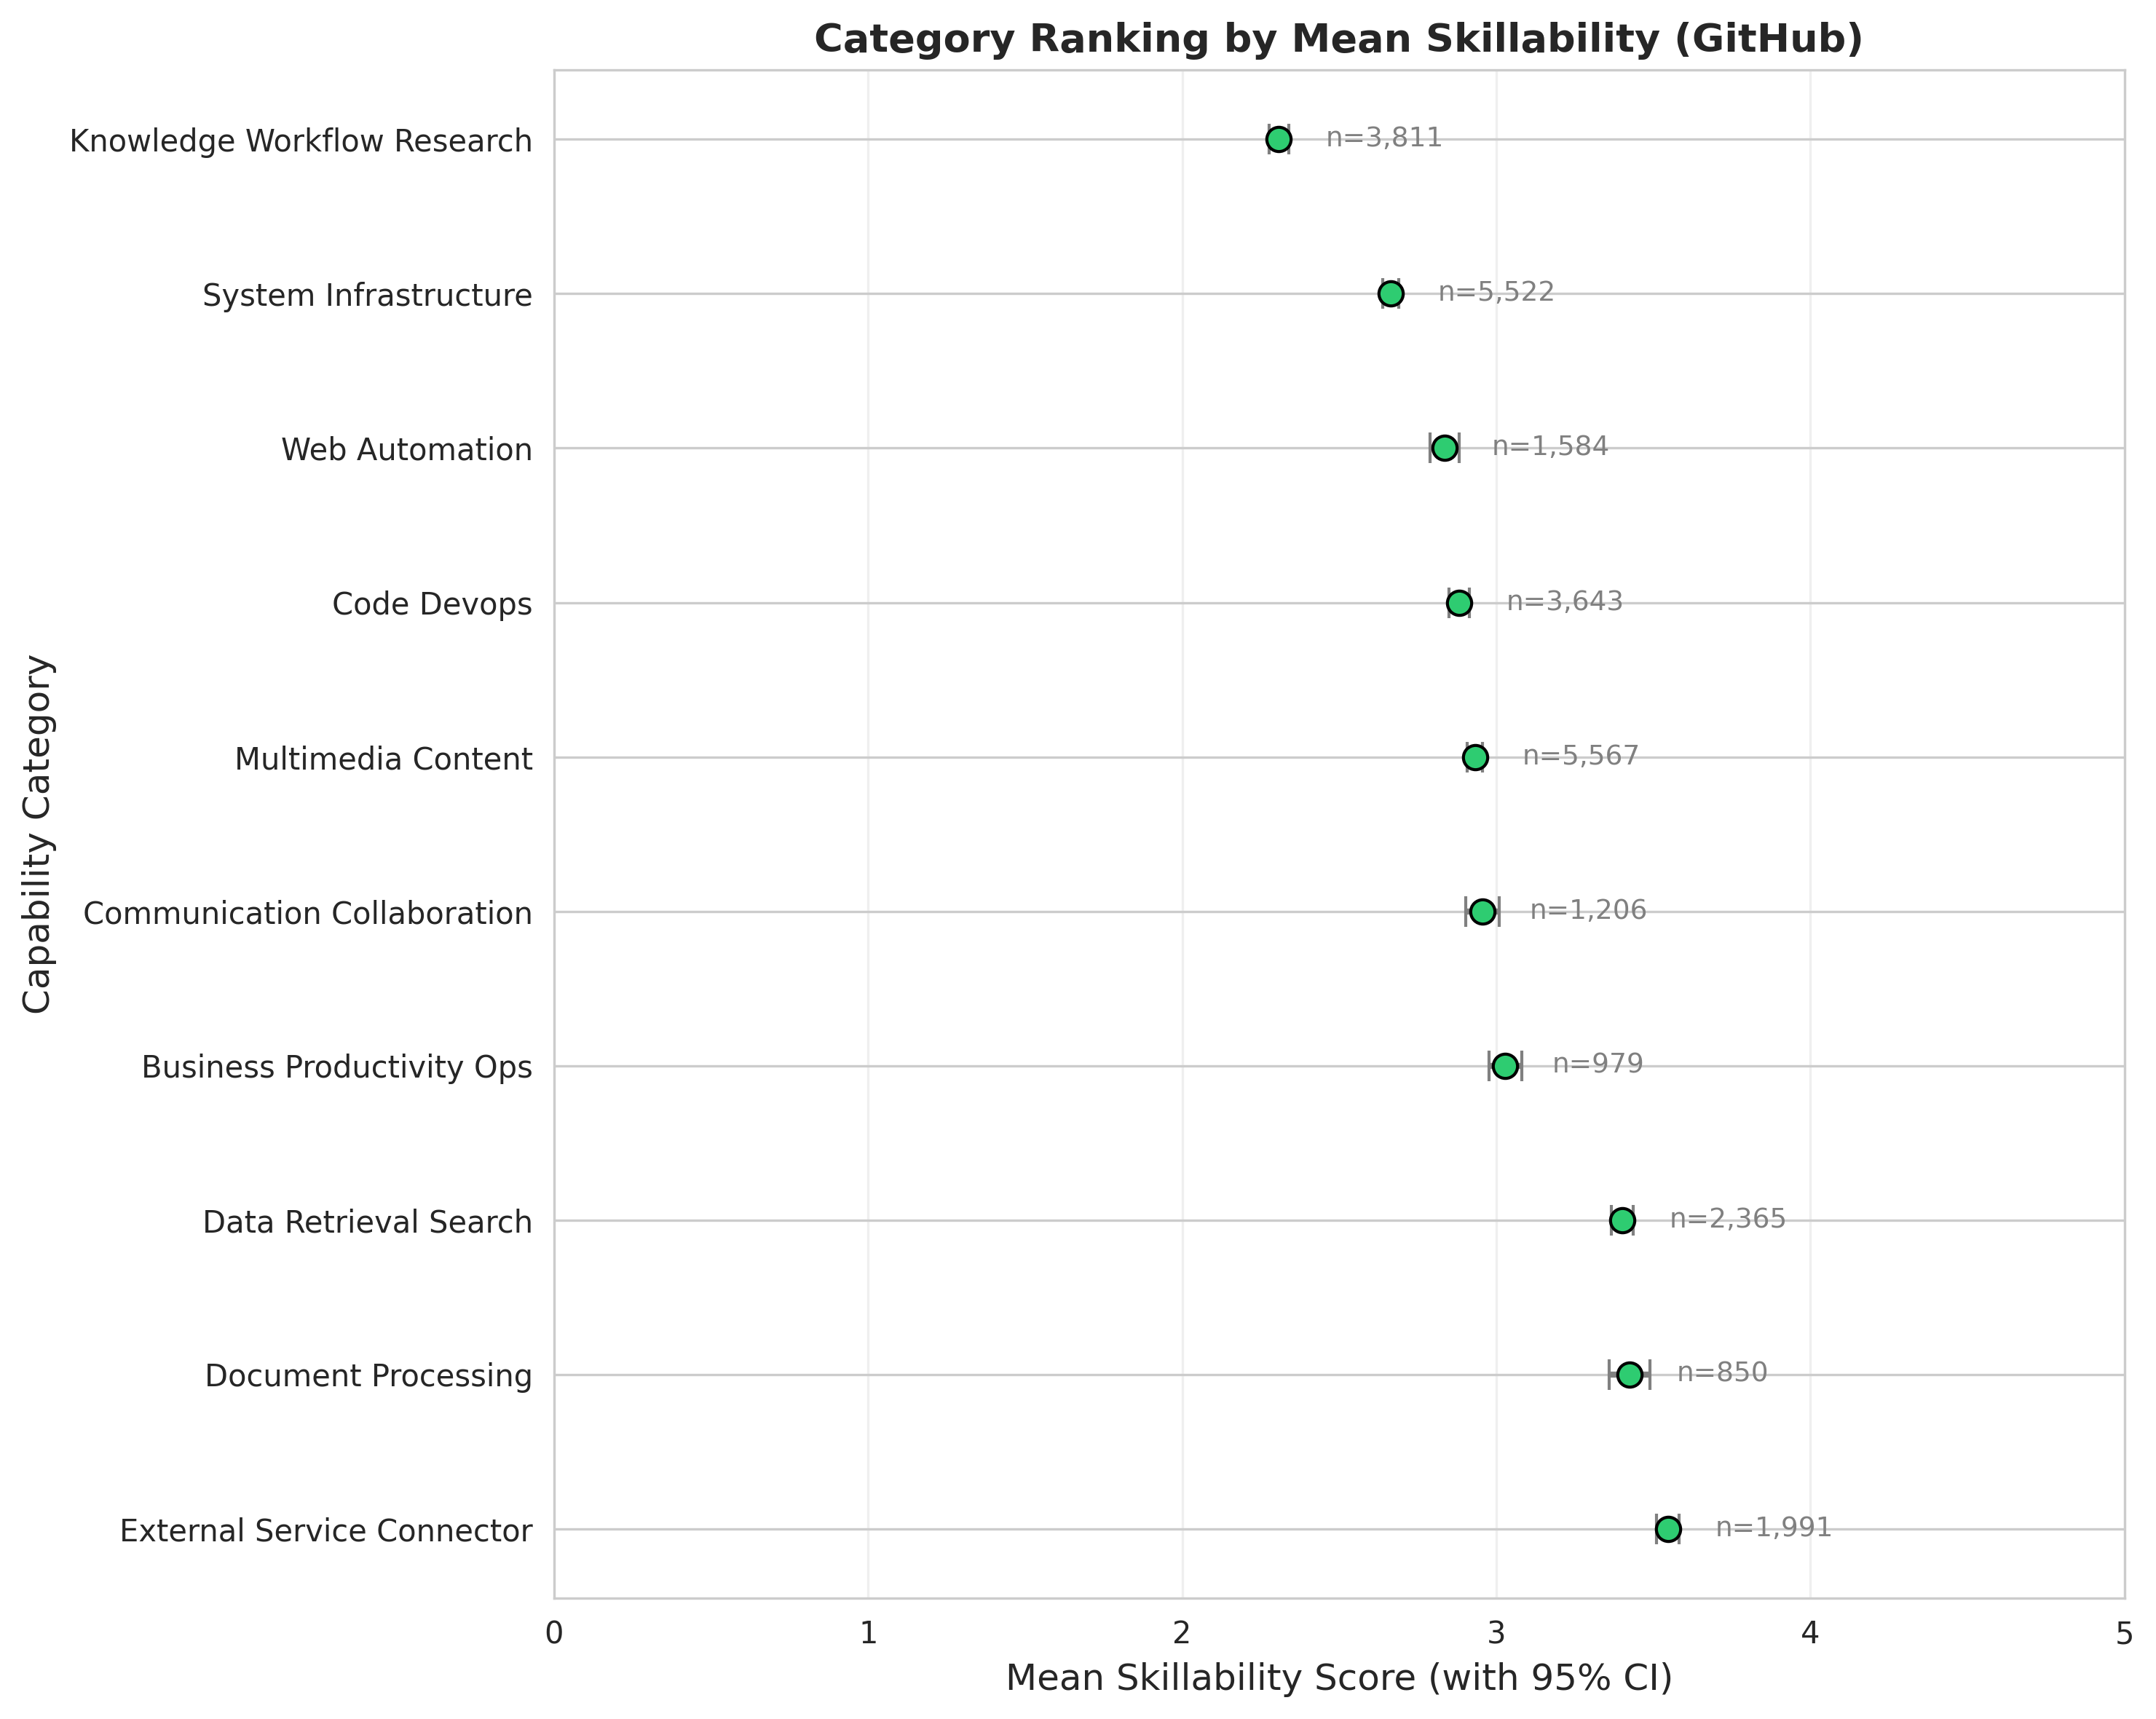
\includegraphics[width=\linewidth]{fig_new2_category_ranking.png}
    \caption{Capability categories ranked by mean skillability in the GitHub sample, with 95\% confidence intervals.}
    \Description{Ranked category plot showing mean skillability and confidence intervals for GitHub capability categories.}
    \label{fig:categories}
\end{figure}

Figure~\ref{fig:categories} ranks the categories with uncertainty bands. The high-opportunity portion of the repository landscape is structured rather than diffuse, which means future large-scale skillification efforts can begin from a relatively clear empirical target map.

\begin{table*}[t]
\caption{Capability-category distribution in the GitHub sample}
\label{tab:categories}
\centering
\begin{tabular}{lrrrrrr}
\toprule
Category & Count & \% & Mean \sscore & SD & High-\skillability \% & Cohen's $d$ vs.\ GitHub overall \\
\midrule
Data Retrieval \& Search & 2,365 & 8.5 & 3.42 & 1.08 & 48.3 & 0.40 \\
Multimedia Content & 5,567 & 20.1 & 3.38 & 1.12 & 46.1 & 0.36 \\
System Infrastructure & 5,522 & 19.9 & 3.31 & 1.15 & 44.2 & 0.36 \\
Document Processing & 850 & 3.1 & 3.28 & 1.09 & 43.8 & 0.34 \\
Web Automation & 1,584 & 5.7 & 3.19 & 1.14 & 41.2 & 0.26 \\
Communication \& Collaboration & 1,206 & 4.4 & 3.15 & 1.11 & 40.1 & 0.23 \\
Code \& DevOps & 3,643 & 13.2 & 3.08 & 1.21 & 38.4 & 0.17 \\
Business \& Productivity & 979 & 3.5 & 2.94 & 1.18 & 34.2 & 0.05 \\
Knowledge \& Workflow & 3,811 & 13.8 & 2.87 & 1.22 & 32.1 & -0.01 \\
External Service Connectors & 1,991 & 7.2 & 2.71 & 1.16 & 28.9 & -0.14 \\
Other & 178 & 0.6 & 2.65 & 1.25 & 27.3 & -0.19 \\
\bottomrule
\end{tabular}
\end{table*}

These category-level results support a simple interpretation: high-\skillability artifacts are most common where tasks are bounded, interfaces are explicit, and automation value is obvious. Data access tools, media processing libraries, and infrastructure utilities fit that profile well. By contrast, connector-style projects often inherit authentication, rate limiting, and external dependency complexity that makes fully autonomous use less straightforward.

\begin{figure}[t]
    \centering
    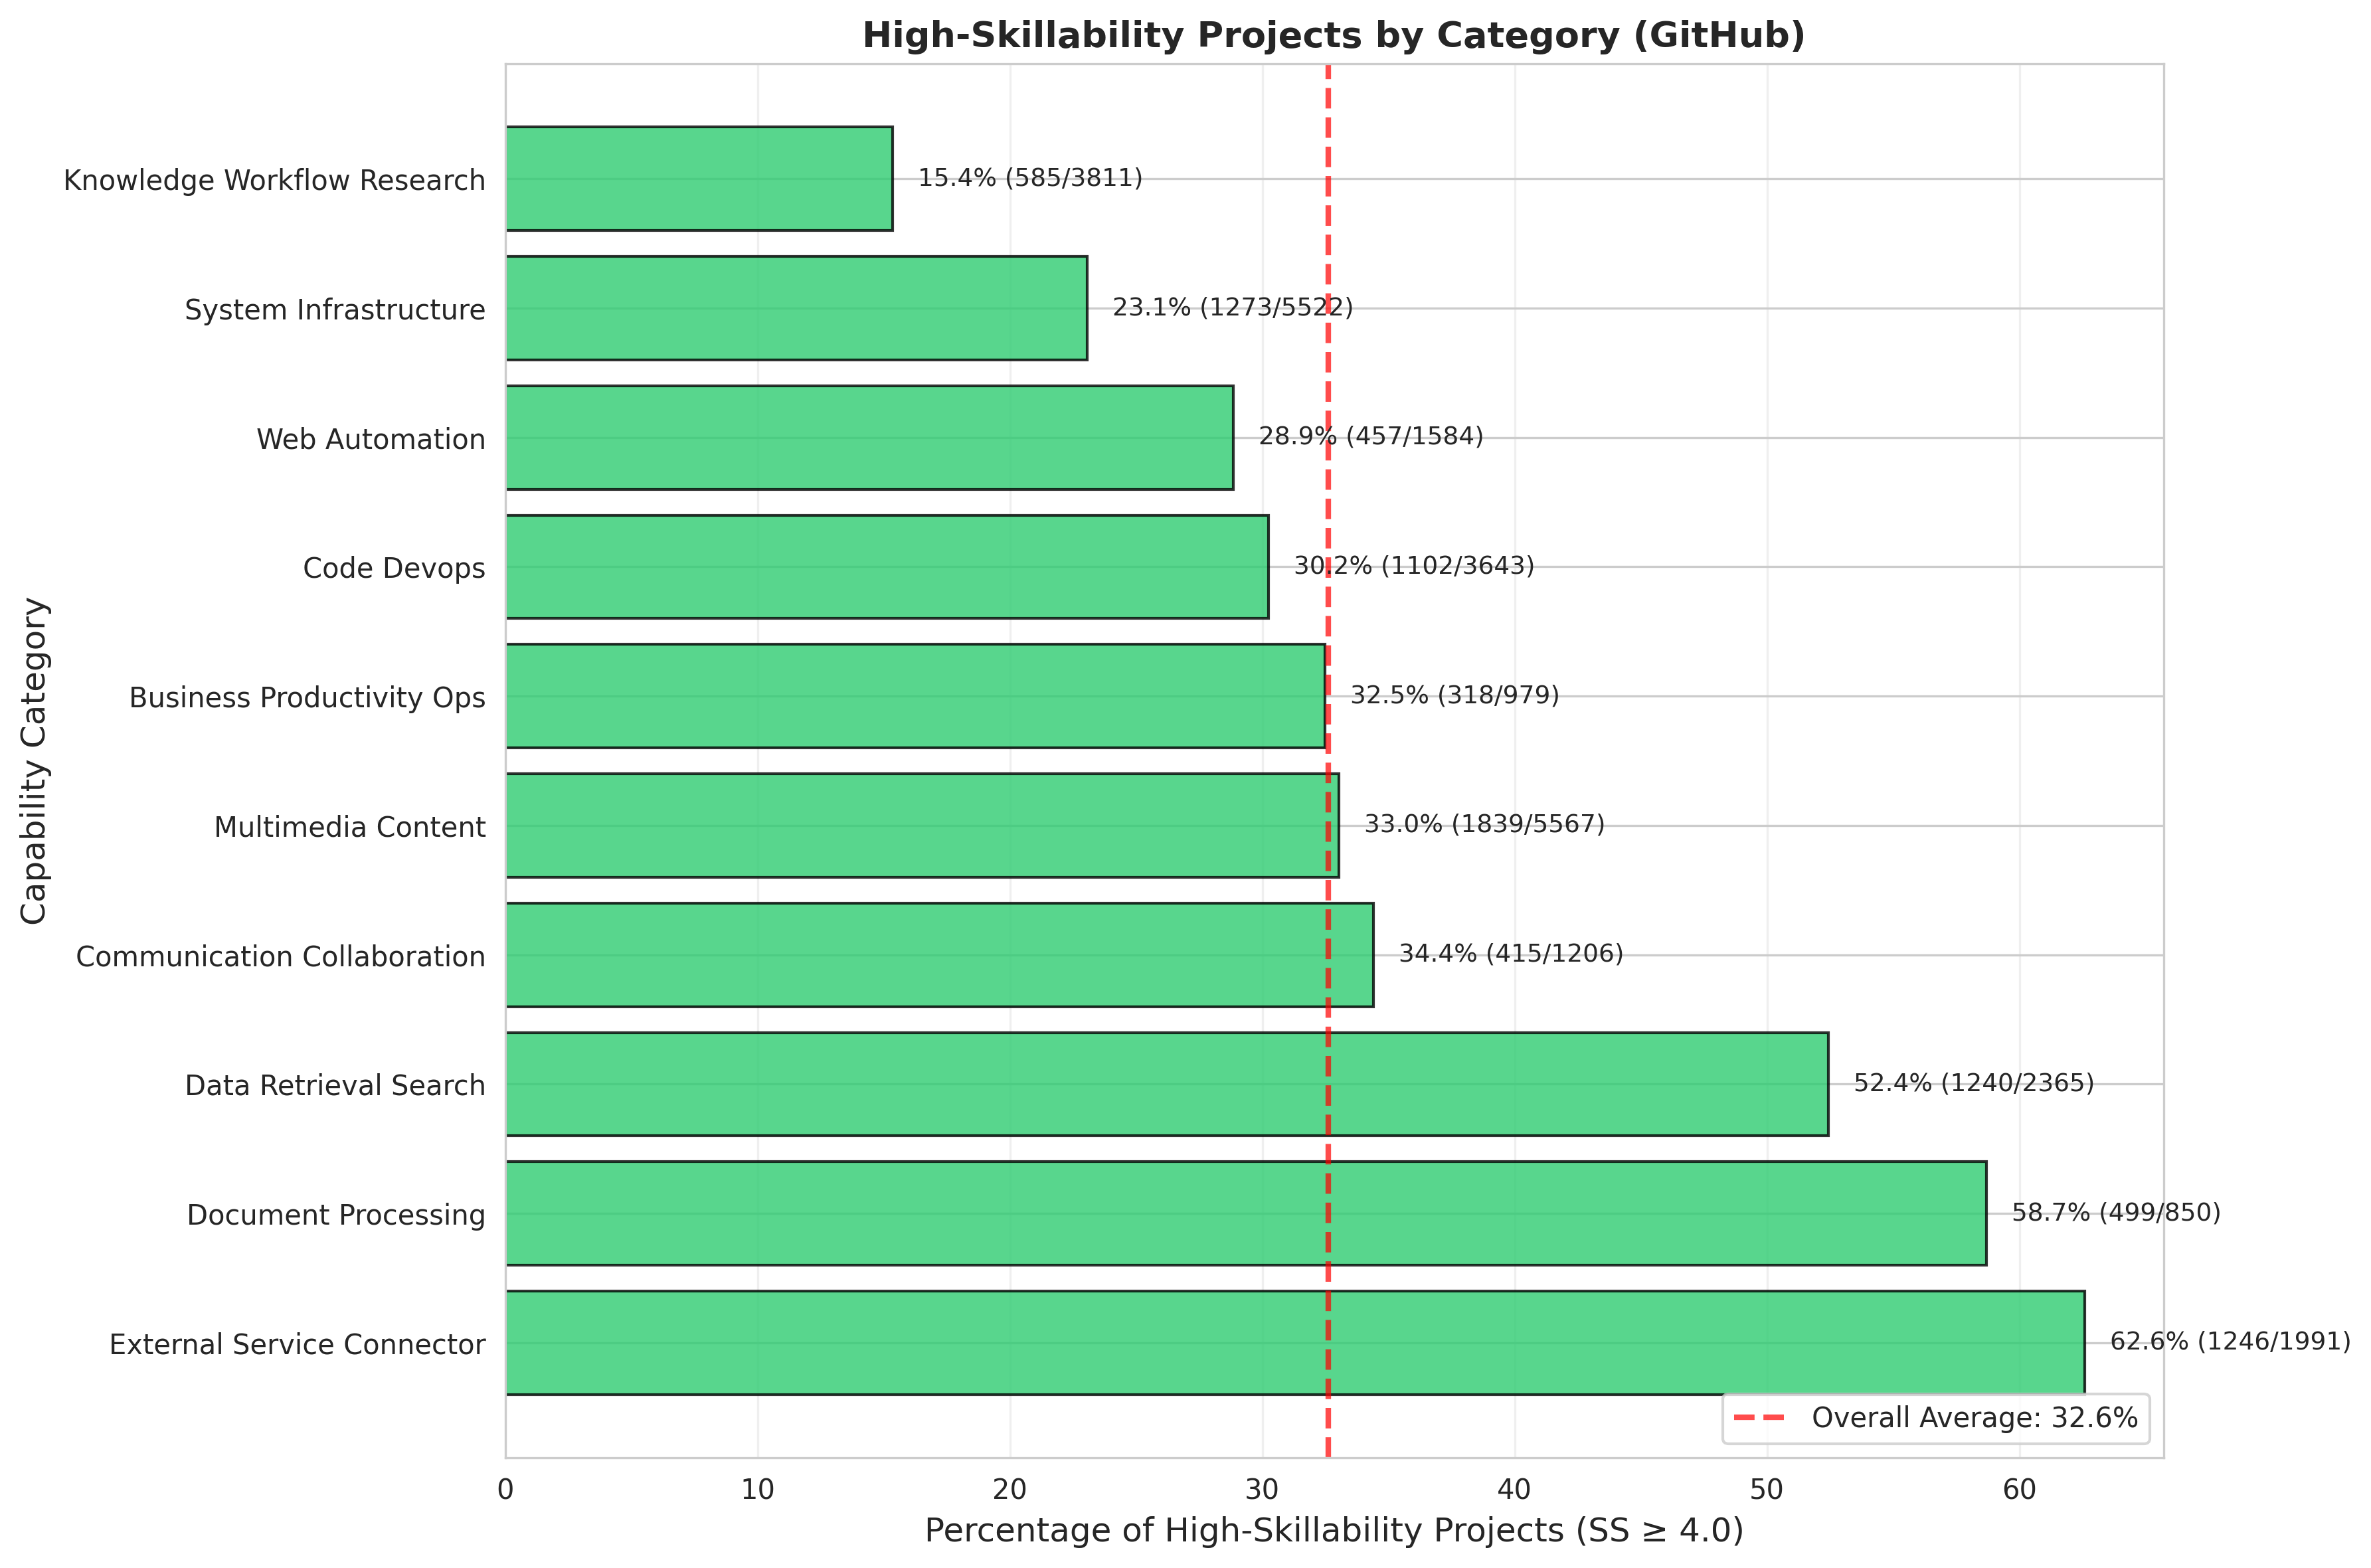
\includegraphics[width=\linewidth]{fig_new3_high_skillability_by_category.png}
    \caption{Share of high-skillability repositories (\(\sscore \ge 4.0\)) by capability category in the GitHub sample.}
    \Description{Bar chart showing the proportion of high-skillability repositories in each GitHub capability category.}
    \label{fig:highskill}
\end{figure}

Figure~\ref{fig:highskill} shows the same result from a thresholded perspective. This view is useful if the goal is to estimate where a practical conversion pipeline is likely to yield many viable skills with limited screening overhead.

Language effects are present but smaller than category effects. Python (mean \sscore = 3.12), Go (3.08), and TypeScript (3.05) score slightly higher than Java (2.87) and C++ (2.71), plausibly because they are common in tooling, automation, and infrastructure domains. Artifact granularity shows a clearer pattern: primitive tools (mean \sscore = 3.45) are stronger candidates than service wrappers (3.21), workflow skills (3.08), and platform adapters (2.87).

\subsection{RQ4: Promising Repositories for Skill Transformation}

Applying \(\sscore \ge 4.0\) together with \(\mathrm{OpportunityScore} \ge 0.7\) yields 9,033 GitHub repositories that we consider promising skill-conversion candidates. This is the most practically consequential result of the paper: even under a conservative ranking rule, the open-source ecosystem appears to contain a substantial inventory of repositories that could plausibly be transformed into agent skills at scale.

The score distribution is as follows: 1,247 repositories (4.5\%) have OpportunityScore at least 0.9; 2,891 (10.4\%) fall in the 0.8--0.9 range; 4,895 (17.7\%) fall in the 0.7--0.8 range; and 18,663 (67.4\%) remain below 0.7.

\begin{figure}[t]
    \centering
    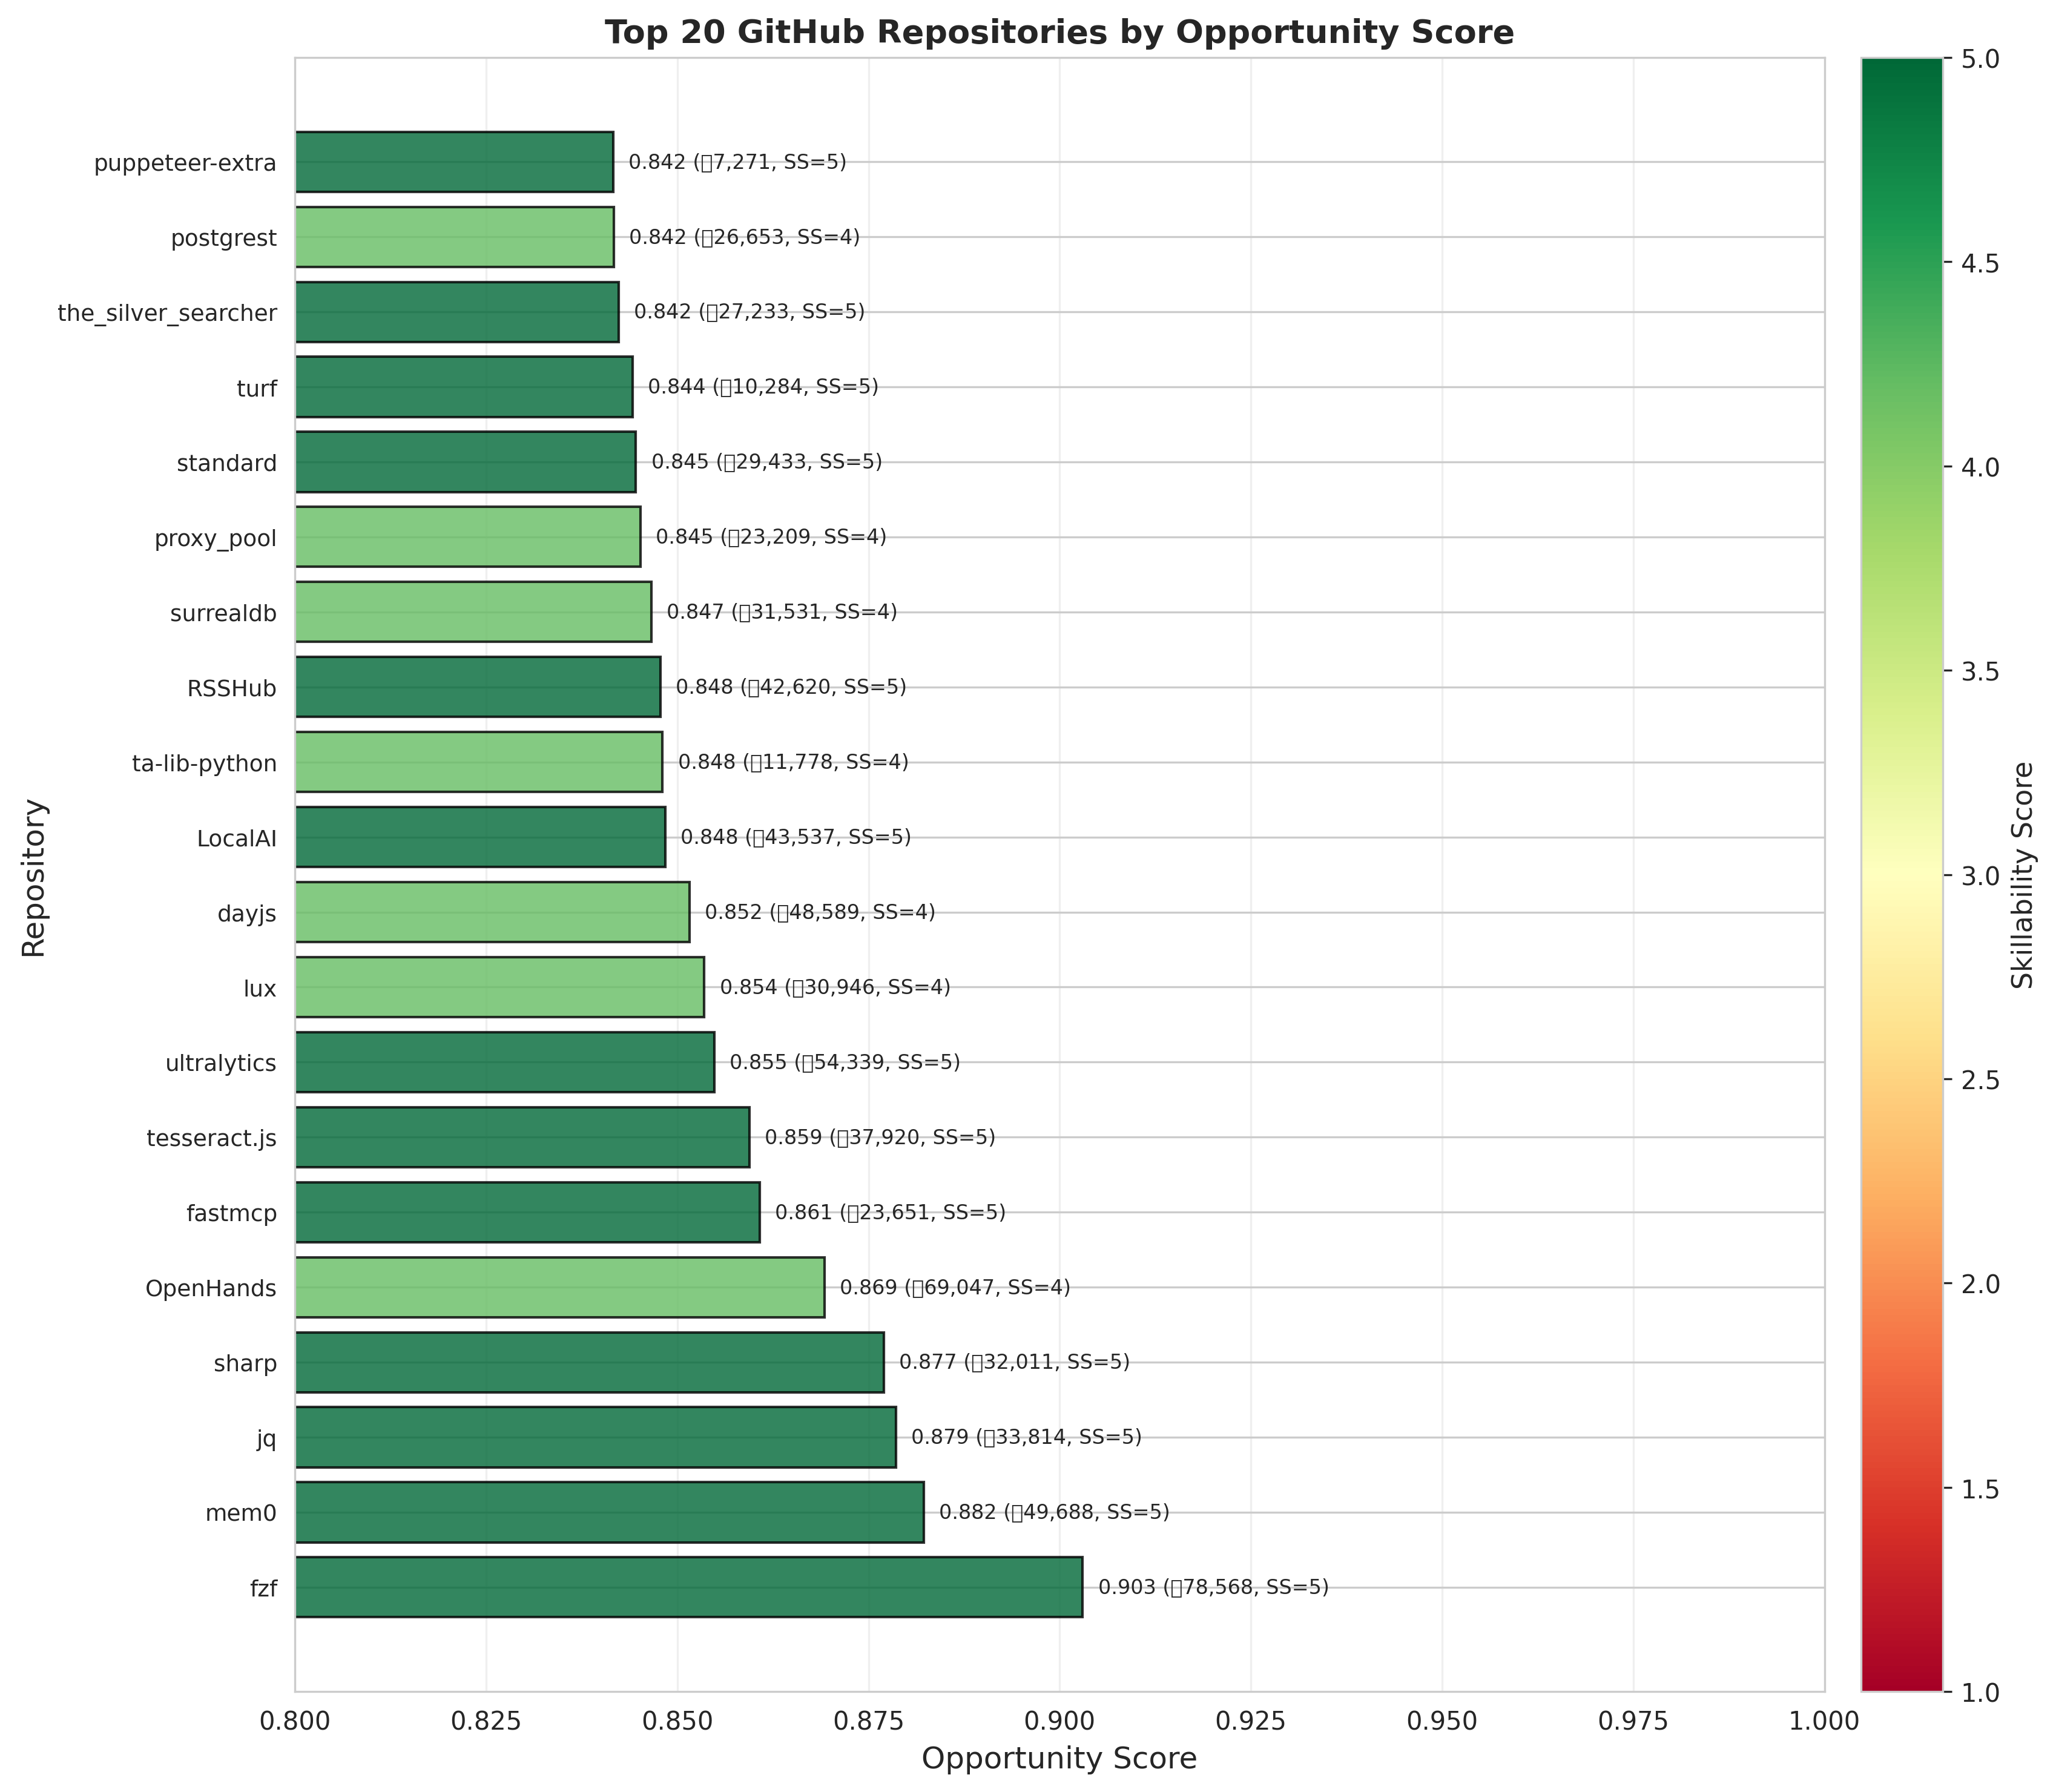
\includegraphics[width=\linewidth]{fig_new4_top_opportunities.png}
    \caption{Top-ranked GitHub repositories by opportunity score.}
    \Description{Ranking chart of top GitHub repositories by opportunity score.}
    \label{fig:topopps}
\end{figure}

Figure~\ref{fig:topopps} makes this opportunity space concrete by showing the top-ranked repositories. The candidate set is not abstract, but already contains recognizable and practically valuable software that could anchor future batch skillification experiments.

\begin{table*}[t]
\caption{Selected high-opportunity repositories}
\label{tab:toprepos}
\centering
\begin{tabularx}{\textwidth}{lXrrrX}
\toprule
Category & Repository & Stars & \sscore & Opp.\ score & Why it appears promising \\
\midrule
Data Retrieval \& Search & \texttt{junegunn/fzf} & 78,568 & 5.00 & 0.903 & Focused CLI tool, clear stdin/stdout model, deterministic local execution \\
Data Retrieval \& Search & \texttt{jqlang/jq} & 33,814 & 5.00 & 0.879 & Declarative JSON transformation, strong composability, minimal side effects \\
Multimedia Content & \texttt{lovell/sharp} & 32,011 & 5.00 & 0.877 & Clear API for image processing, strong automation value, predictable outputs \\
Multimedia Content & \texttt{ultralytics/ultralytics} & 54,339 & 5.00 & 0.855 & Structured computer-vision workflows exposed through documented interfaces \\
System Infrastructure & \texttt{giampaolo/psutil} & 10,000 & 4.75 & 0.860 & Typed system-inspection API with obvious monitoring and automation uses \\
Document Processing & \texttt{naptha/tesseract.js} & 37,920 & 5.00 & 0.859 & Self-contained OCR with clear inputs, outputs, and confidence scores \\
Code \& DevOps & \texttt{OpenHands/OpenHands} & 69,047 & 4.00 & 0.869 & Strong automation relevance and explicit interfaces, despite larger scope \\
External Service Connectors & \texttt{PrefectHQ/fastmcp} & 23,651 & 5.00 & 0.861 & Explicit schema generation and tool-wrapping support for agent ecosystems \\
Knowledge \& Workflow & \texttt{mem0ai/mem0} & 49,688 & 5.00 & 0.882 & Focused memory abstraction with clear agent-facing use cases \\
\bottomrule
\end{tabularx}
\end{table*}

Popularity is a poor proxy for raw \skillability. In the GitHub sample, the correlation between \skillability and stars is effectively zero (\(r_s = 0.003\), \(p = 0.62\)). A repository-to-skill pipeline that relies only on popularity signals would therefore overlook a large share of the available opportunity space.

\begin{figure}[t]
    \centering
    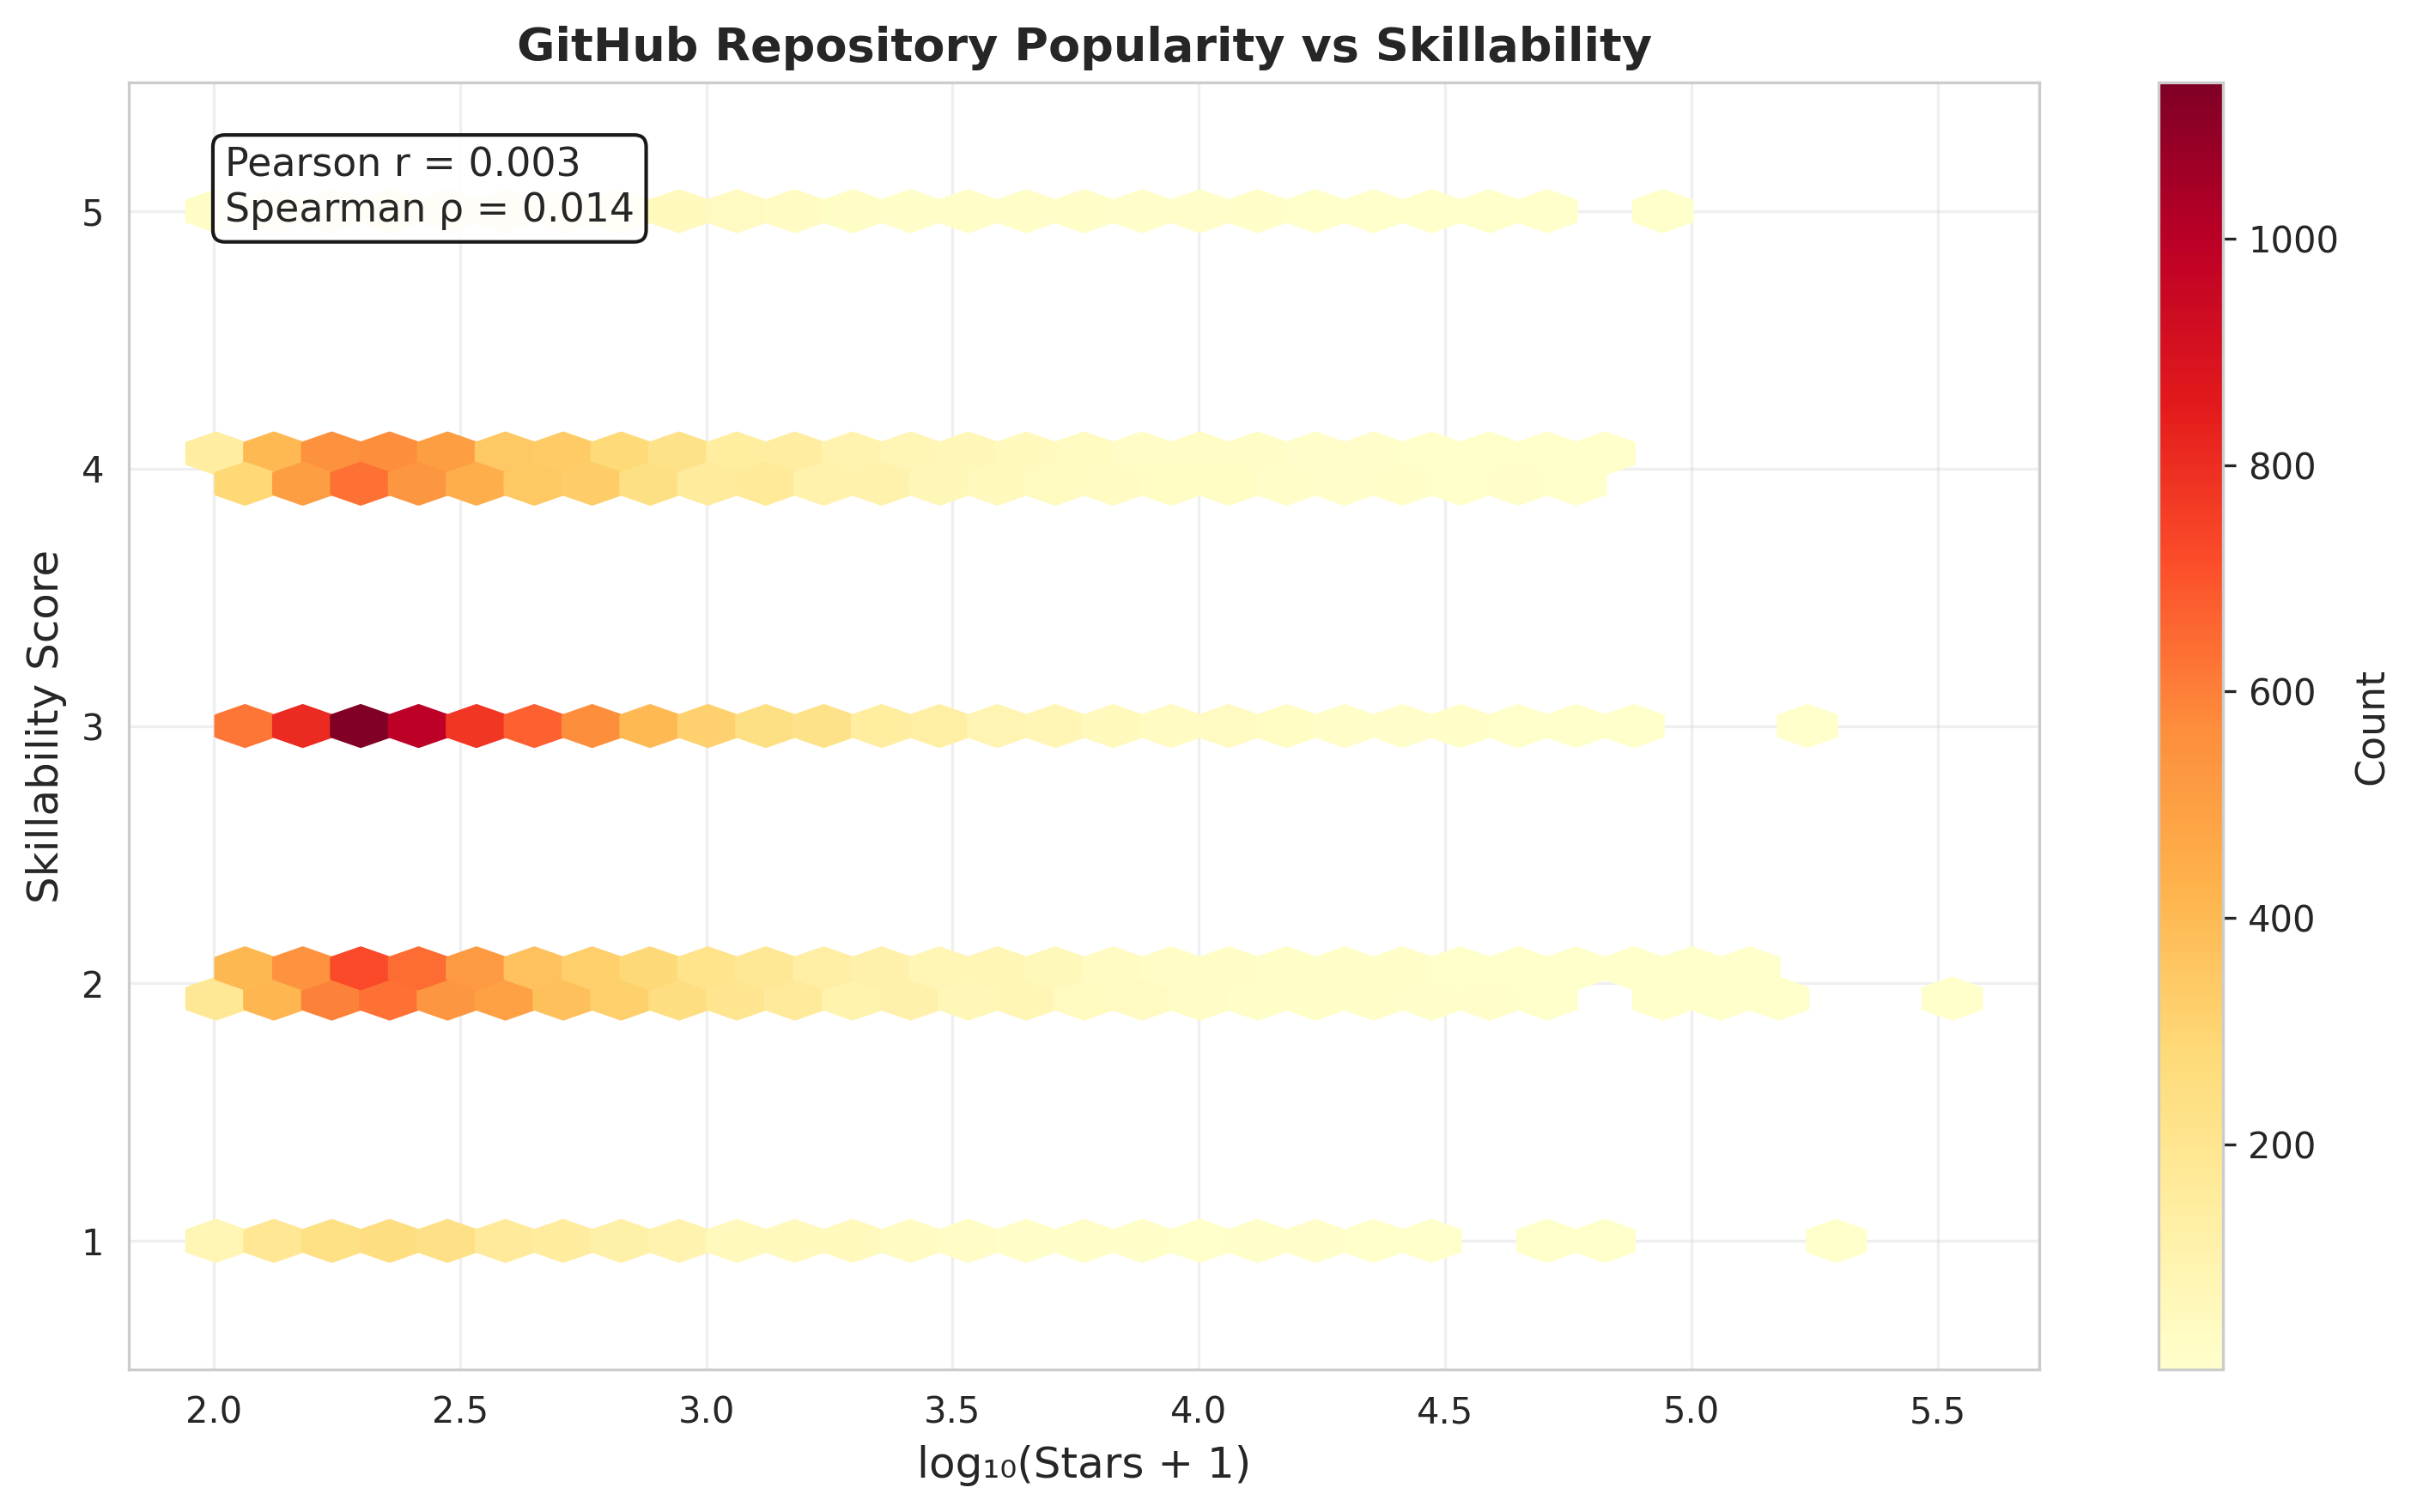
\includegraphics[width=\linewidth]{fig8_stars_vs_skillability.png}
    \caption{Skillability scores versus GitHub stars (log scale) for sampled repositories.}
    \Description{Scatter plot of GitHub stars versus skillability scores for sampled repositories.}
    \label{fig:stars}
\end{figure}

Figure~\ref{fig:stars} visualizes this disconnect directly. High-\skillability repositories appear across the full popularity range, including many projects far below the top-starred tier. By contrast, the correlation between OpportunityScore and stars is weakly positive (\(r_s = 0.138\), \(p < 0.001\)) because stars are intentionally included in the ranking heuristic.

\subsection{Supplementary Check: Discriminating Marketplace Membership}

As a supplementary analysis, we trained binary classifiers to distinguish Clawhub skills from GitHub repositories. The goal is modest: to test whether the \skillability features carry useful signal beyond simple repository metadata. This is not an adoption study in the causal sense, because marketplace membership also reflects curation policy, documentation format, and platform-specific packaging decisions.

Using only basic metadata (\texttt{has\_license}, \texttt{archived}), XGBoost achieved AUC = 0.8801 (95\% CI [0.8701, 0.8901]). Adding the six \skillability dimensions plus taxonomy features increased performance to AUC = 0.9863 (95\% CI [0.9831, 0.9894]) and improved PR-AUC from 0.2489 to 0.8360. SHAP and ablation analyses consistently ranked Automation Value, Composability, and Task Clarity as the most informative features. We interpret this result narrowly: the construct appears to align with the practical distinctions that separate marketplace artifacts from general repositories.

\section{Discussion}

\subsection{What the Results Suggest}

Three findings appear most robust. First, the space of agent-friendly software is non-trivial. Even under a conservative and imperfect measurement process, roughly one third of the analyzed corpus crosses the high-\skillability threshold. That suggests not just headroom for better curation, but the feasibility of a broader pipeline in which repositories are discovered, screened, wrapped, and published as skills in a much more systematic way than current marketplace practice.

Second, the most promising candidates are not distributed uniformly across software domains. Repository categories centered on focused transformations, data access, media processing, and system inspection contain the densest pockets of promising artifacts. This gives future work an empirical map of where batch skillification efforts are most likely to succeed first.

Third, popularity and \skillability are not the same thing. The near-zero star correlation suggests that common open-source visibility signals are poorly aligned with the specific needs of agent-facing reuse. Curation strategies that simply rank by stars are therefore likely to miss many viable skill candidates, whereas a dedicated discovery layer can surface a much larger conversion frontier.

\subsection{Implications}

\textbf{For marketplace operators.} A rubric like \skillability can support not only first-pass scouting, but also staged acquisition pipelines: identify candidates, prioritize them by expected conversion payoff, and focus packaging resources on categories with the highest expected yield. The current results suggest starting with data retrieval, multimedia, document processing, and infrastructure-heavy categories, where focused automation value is common.

\textbf{For repository maintainers.} Projects that aim to be agent-friendly should optimize for focused scope, explicit interfaces, deterministic behavior where possible, and operationally safe defaults. Better documentation matters not only for humans, but also for machine-mediated reuse.

\textbf{For tool and agent platform designers.} The strong separation on automation value and composability suggests that wrapper generation, schema extraction, execution isolation, and deployment templating are especially important leverage points. Tools that reduce packaging overhead could turn high-\skillability repositories into skills in semi-automated or even batch-oriented ways.

\textbf{For researchers.} The paper does not end the measurement question; it opens a broader pipeline question. A promising next step is to connect repository-level annotations to downstream agent task outcomes, tool-call success, wrapping effort, and marketplace adoption so that the field can move from descriptive ranking to end-to-end repository-to-skill engineering.

\subsection{Threats to Validity}

\textbf{Construct validity.} \skillability is an exploratory construct defined by our rubric and weighting choices. Although the dimensions are grounded in software reuse and agent-tool requirements, they are not yet validated through factor analysis, expert consensus methods, or external outcome measures. The \(\sscore \ge 4.0\) threshold is also heuristic.

\textbf{Internal validity.} The comparison between Clawhub and GitHub is confounded by curation, documentation format, and artifact scope. The supplementary classifier may partially exploit the same differences. These analyses therefore support descriptive and discriminative claims, not causal ones.

\textbf{Conclusion validity.} We report effect sizes and confidence intervals, and we use rank-based correlation where the data are highly skewed. Even so, the analyses inherit measurement error from the annotation pipeline. Because the study is exploratory, we do not apply family-wise multiple-testing corrections and avoid strong confirmatory interpretations.

\textbf{External validity.} Our GitHub sampling frame excludes very new, low-visibility, undocumented, or archived repositories. The results therefore generalize to a more practical but narrower population: actively maintained and documented open-source projects with some level of community validation.

\textbf{Annotation validity.} The LLM sees repository metadata and README excerpts rather than code, tests, dependency graphs, or runtime behavior. As a result, scores for interface clarity, deployment friction, and operational risk can be wrong in either direction. The 200-item validation study provides useful evidence of approximate alignment, but not full annotation reliability.

\subsection{Future Work}

We see four concrete next steps:
\begin{enumerate}[leftmargin=*,itemsep=2pt]
    \item \textbf{Stronger construct validation.} Expert panels, factor analysis, and agreement studies with multiple human annotators could test whether the six dimensions hold together as intended.
    \item \textbf{Outcome-based validation.} The most important follow-up is to correlate \skillability with downstream agent performance: tool-call success, task completion, failure recovery, wrapping effort, and user-perceived utility.
    \item \textbf{Batch skillification pipelines.} A natural next step is to build and evaluate end-to-end workflows that take high-\skillability repositories, generate wrappers and interface schemas, provision execution environments, and measure how many can be converted into usable skills with limited human intervention.
    \item \textbf{Richer evidence sources and matched studies.} Future versions should incorporate code structure, API schemas, tests, dependency graphs, container metadata, and security signals rather than README text alone.
\end{enumerate}

\section{Conclusion}

This paper investigated how open-source software can be characterized for transformation into agent-facing skills. We introduced \skillability as an exploratory six-dimensional construct and applied it to 29,896 artifacts spanning both a skill marketplace and GitHub. The study shows that marketplace artifacts and general repositories occupy different regions of the \skillability space, that high-\skillability candidates are concentrated in a few capability domains, and that repository popularity is a poor proxy for raw skill-conversion potential.

The main claim of the paper is forward-looking: repository-scale discovery of promising skill candidates is feasible, the candidate pool is large enough to matter, and the opportunity space is structured enough to support targeted conversion strategies. In that sense, this work serves as a front-end stage for future repository-to-skill pipelines. It identifies where large-scale or semi-automated skillification is most plausible, what classes of repositories should be prioritized first, and which technical bottlenecks future systems should attack.

We do not present \skillability as a finished measurement instrument. We present it as a useful and scalable empirical basis for the next phase of research: moving from repository mining and candidate ranking toward end-to-end systems that can discover, wrap, evaluate, and publish skills in bulk.

\appendix

\section{Annotation Rubric Summary}

Each artifact was annotated with a prompt containing (1) a system instruction defining the six \skillability dimensions with 1--5 anchors, (2) artifact metadata, (3) a README excerpt capped at 3,000 characters, and (4) a JSON schema requiring six numeric dimension scores plus category, granularity, and execution-mode labels.

\begin{table}[h]
\caption{Human spot-validation agreement}
\centering
\begin{tabular}{lr}
\toprule
Dimension & Agreement \\
\midrule
Task Clarity & 89\% \\
Interface Clarity & 85\% \\
Composability & 84\% \\
Automation Value & 91\% \\
Deployment Friction & 86\% \\
Operational Risk & 88\% \\
Overall & 87\% \\
\bottomrule
\end{tabular}
\end{table}

\section{Supplementary Numerical Summary}

\begin{itemize}[leftmargin=*]
    \item Total analyzed artifacts: 29,896
    \item High-\skillability artifacts overall: 10,698 (35.8\%)
    \item Clawhub mean \sscore: 3.75
    \item GitHub mean \sscore: 2.88
    \item Mean difference: 0.87, 95\% CI [0.81, 0.93], Cohen's $d = 0.74$
    \item GitHub repositories satisfying \(\sscore \ge 4.0\) and \(\mathrm{OpportunityScore} \ge 0.7\): 9,033
    \item \skillability vs.\ stars: \(r_s = 0.003\), \(p = 0.62\)
    \item OpportunityScore vs.\ stars: \(r_s = 0.138\), \(p < 0.001\)
\end{itemize}

\begin{thebibliography}{45}

\bibitem{ref1}
Wang, L., Ma, C., Feng, X., et al. 2024. A Survey on Large Language Model based Autonomous Agents. \textit{Frontiers of Computer Science} 18, 6, 186345.

\bibitem{ref2}
Qian, C., Cong, X., Yang, C., et al. 2023. Communicative Agents for Software Development. \textit{arXiv preprint arXiv:2307.07924}.

\bibitem{ref3}
GitHub. 2024. The State of the Octoverse 2024. GitHub Blog. \url{https://github.blog/news-insights/octoverse/}

\bibitem{ref4}
McIlroy, M. D. 1968. Mass Produced Software Components. In \textit{Software Engineering: Report on a Conference}. NATO Science Committee, 138--155.

\bibitem{ref5}
Szyperski, C. 2002. \textit{Component Software: Beyond Object-Oriented Programming}. Addison-Wesley.

\bibitem{ref6}
Heineman, G. T. and Councill, W. T. 2001. \textit{Component-Based Software Engineering: Putting the Pieces Together}. Addison-Wesley.

\bibitem{ref7}
Crnkovic, I., Sentilles, S., Vulgarakis, A., and Chaudron, M. R. 2011. A Classification Framework for Software Component Models. \textit{IEEE Transactions on Software Engineering} 37, 5, 593--615.

\bibitem{ref8}
Frakes, W. B. and Kang, K. 2005. Software Reuse Research: Status and Future. \textit{IEEE Transactions on Software Engineering} 31, 7, 529--536.

\bibitem{ref9}
Krueger, C. W. 1992. Software Reuse. \textit{ACM Computing Surveys} 24, 2, 131--183.

\bibitem{ref10}
Morisio, M., Ezran, M., and Tully, C. 2002. Success and Failure Factors in Software Reuse. \textit{IEEE Transactions on Software Engineering} 28, 4, 340--357.

\bibitem{ref11}
Pohl, K., Bockle, G., and van der Linden, F. J. 2005. \textit{Software Product Line Engineering}. Springer.

\bibitem{ref12}
Apel, S. and Kastner, C. 2009. An Overview of Feature-Oriented Software Development. \textit{Journal of Object Technology} 8, 5, 49--84.

\bibitem{ref13}
Manikas, K. and Hansen, K. M. 2013. Software Ecosystems -- A Systematic Literature Review. \textit{Journal of Systems and Software} 86, 5, 1294--1306.

\bibitem{ref14}
Bosch, J. 2009. From Software Product Lines to Software Ecosystems. In \textit{SPLC}. 111--119.

\bibitem{ref15}
Kagdi, H., Collard, M. L., and Maletic, J. I. 2007. A Survey and Taxonomy of Approaches for Mining Software Repositories in the Context of Software Evolution. \textit{Journal of Software Maintenance and Evolution} 19, 2, 77--131.

\bibitem{ref16}
Hassan, A. E. 2008. The Road Ahead for Mining Software Repositories. In \textit{FoSM}. 48--57.

\bibitem{ref17}
Dyer, R., Nguyen, H. A., Rajan, H., and Nguyen, T. N. 2013. Boa: A Language and Infrastructure for Analyzing Ultra-Large-Scale Software Repositories. In \textit{ICSE}. 422--431.

\bibitem{ref18}
Borges, H., Hora, A., and Valente, M. T. 2016. Understanding the Factors That Impact the Popularity of GitHub Repositories. In \textit{ICSME}. 334--344.

\bibitem{ref19}
Munaiah, N., Kroh, S., Cabrey, C., and Nagappan, M. 2017. Curating GitHub for Engineered Software Projects. \textit{Empirical Software Engineering} 22, 6, 3219--3253.

\bibitem{ref20}
Decan, A., Mens, T., and Grosjean, P. 2019. An Empirical Comparison of Dependency Network Evolution in Seven Software Packaging Ecosystems. \textit{Empirical Software Engineering} 24, 1, 381--416.

\bibitem{ref21}
Kikas, R., Gousios, G., Dumas, M., and Pfahl, D. 2017. Structure and Evolution of Package Dependency Networks. In \textit{MSR}. 102--112.

\bibitem{ref22}
Piccioni, M., Furia, C. A., and Meyer, B. 2013. An Empirical Study of API Usability. In \textit{ESEM}. 5--14.

\bibitem{ref23}
Stylos, J. and Myers, B. A. 2008. The Implications of Method Placement on API Learnability. In \textit{FSE}. 105--112.

\bibitem{ref24}
Ellis, B., Stylos, J., and Myers, B. 2007. The Factory Pattern in API Design: A Usability Evaluation. In \textit{ICSE}. 302--312.

\bibitem{ref25}
Myers, B. A. and Stylos, J. 2016. Improving API Usability. \textit{Communications of the ACM} 59, 6, 62--69.

\bibitem{ref26}
Robillard, M. P. 2009. What Makes APIs Hard to Learn? Answers from Developers. \textit{IEEE Software} 26, 6, 27--34.

\bibitem{ref27}
Schick, T., Dwivedi-Yu, J., Dessi, R., et al. 2023. Toolformer: Language Models Can Teach Themselves to Use Tools. In \textit{NeurIPS}. 68539--68551.

\bibitem{ref28}
Yao, S., Zhao, J., Yu, D., et al. 2023. ReAct: Synergizing Reasoning and Acting in Language Models. In \textit{ICLR}.

\bibitem{ref29}
Patil, S. G., Zhang, T., Wang, X., and Gonzalez, J. E. 2023. Gorilla: Large Language Model Connected with Massive APIs. \textit{arXiv preprint arXiv:2305.15334}.

\bibitem{ref30}
Significant Gravitas. 2023. AutoGPT: An Experimental Open-Source Attempt to Make GPT-4 Fully Autonomous. GitHub Repository. \url{https://github.com/Significant-Gravitas/AutoGPT}

\bibitem{ref31}
Chase, H. 2022. LangChain: Building Applications with LLMs through Composability. GitHub Repository. \url{https://github.com/langchain-ai/langchain}

\bibitem{ref32}
Anthropic. 2024. Claude Tool Use Documentation. Anthropic Developer Documentation. \url{https://docs.anthropic.com/claude/docs/tool-use}

\bibitem{ref33}
Qin, Y., Liang, S., Ye, Y., et al. 2023. ToolLLM: Facilitating Large Language Models to Master 16000+ Real-world APIs. \textit{arXiv preprint arXiv:2307.16789}.

\bibitem{ref34}
Clawhub. 2024. Clawhub Agent Skill Marketplace. \url{https://clawhub.ai}

\bibitem{ref35}
Anthropic. 2024. Model Context Protocol (MCP): A Standard for Connecting AI Assistants to Data Sources. Anthropic Blog. \url{https://www.anthropic.com/news/model-context-protocol}

\bibitem{ref36}
Martin, W., Sarro, F., Jia, Y., Zhang, Y., and Harman, M. 2017. A Survey of App Store Analysis for Software Engineering. \textit{IEEE Transactions on Software Engineering} 43, 9, 817--847.

\bibitem{ref37}
Harman, M., Jia, Y., and Zhang, Y. 2012. App Store Mining and Analysis: MSR for App Stores. In \textit{MSR}. 108--111.

\bibitem{ref38}
Newman, S. 2015. \textit{Building Microservices: Designing Fine-Grained Systems}. O'Reilly.

\bibitem{ref39}
ISO/IEC 25010. 2011. Systems and Software Engineering -- Systems and Software Quality Requirements and Evaluation (SQuaRE) -- System and Software Quality Models.

\bibitem{ref40}
Grady, R. B. and Caswell, D. L. 1987. \textit{Software Metrics: Establishing a Company-Wide Program}. Prentice-Hall.

\bibitem{ref41}
Kitchenham, B., Pfleeger, S. L., and Fenton, N. 1995. Towards a Framework for Software Measurement Validation. \textit{IEEE Transactions on Software Engineering} 21, 12, 929--944.

\bibitem{ref42}
Fenton, N. E. and Bieman, J. 2014. \textit{Software Metrics: A Rigorous and Practical Approach}. CRC Press.

\bibitem{ref43}
Zheng, L., Chiang, W.-L., Sheng, Y., et al. 2023. Judging LLM-as-a-Judge with MT-Bench and Chatbot Arena. In \textit{NeurIPS}. 46595--46623.

\bibitem{ref44}
Kocmi, T. and Federmann, C. 2023. Large Language Models Are State-of-the-Art Evaluators of Translation Quality. In \textit{EAMT}. 193--203.

\bibitem{ref45}
Gilardi, F., Alizadeh, M., and Kubli, M. 2023. ChatGPT Outperforms Crowd-Workers for Text-Annotation Tasks. \textit{Proceedings of the National Academy of Sciences} 120, 30, e2305016120.

\end{thebibliography}

\end{document}
